Kapitel \ref{chp:interaktion_mit_multitoucheingaben} zeigt, dass die gleichzeitige Steuerung aller Freiheitsgrade einer 3D Manipulation durch Multi-Touch Eingaben noch immer eine Herausforderung ist. In Kapitel \ref{chp:explizite_interaktion} werden Lösungsansätze vorgestellt, mit welchen einzelne Freiheitsgrade der Interaktion explizit manipuliert werden können. Ein modulares System zur Koordination dieser Techniken, wäre ein Ansatz mit allen Freiheitsgrade explizit umzugehen. Die Bedienbarkeit eines solchen Systems könnte jedoch schnell komplex werden.
\\\\
Dieses Kapitel beschreibt und evaluiert eine im Rahmen dieser Arbeit entstandene Navigationstechnik namens \emph{Levelling}. Hierzu wird in Abschnitt \ref{sec:definition_levelling} eine Definition zu \emph{impliziter} Navigationstechnik, sowie eine Erklärung zum Interaktionsziel von \emph{Levelling}, gegeben. Im darauf folgenden Abschnitt \ref{sec:depth_levelling} wird die Funktionsweise von \emph{Depth-Levelling} beschrieben, während in Abschnitt \ref{sec:rotation_levelling} auf den erweiterten Ansatz \emph{Rotation-Levelling} eingegangen wird. Abschließend wird in Abschnitt \ref{sec:vorteile_und_limitierungen_implizit} \emph{Levelling} als Navigationstechnik diskutiert.


\section{Definition und Interaktionsziele}
\label{sec:definition_levelling}

Wir definieren implizite Navigationstechniken als zusätzliche Transformationen zur Erreichung eines Interaktionsziels, welche der Anwendung expliziter Techniken beigefügt werden und nicht getrennt von diesen bedienbar sind. 

\begin{figure}
	\begin{center}
		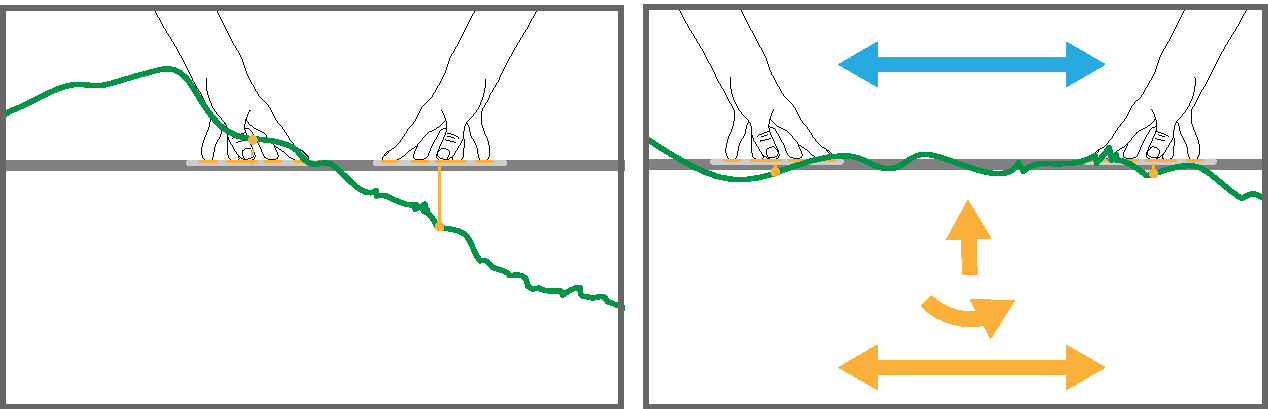
\includegraphics[width=12cm]{img/levelling_concept.pdf}
	\end{center}
	\caption{Visualisierung des \emph{Levelling} Interaktionskonzepts. Die berührte Geometrie wird im Nahfeld des Tisches geebnet.} 
	\label{fig:levelling_concept}
\end{figure}

Bruder et al. \cite{bruder:2013} beschreibt, dass eine effektive Interaktion mit dreidimensionalen Inhalten vor allem möglich ist, wenn Objekte in Null-Parallaxe liegen. \emph{Levelling} ist ein Ansatz zur impliziten Steuerung der Navigation. Ziel der Technik ist es, nutzerdefinierte Applikationsinhalte auf Tischebene zu bewegen und darauf zu ebnen. Es wird dabei sowohl die Distanz der Geometrie zur Bildebene verringert, sowie die Orientierung angepasst. Hierzu legt der Anwender durch Berühren des Projektionstisches mit beiden Händen zwei Auftreffpunkte auf der Geometrie fest, welche durch die \emph{Levelling} Technik schrittweise näher an die Bildschirmfläche geführt werden. Da sich beide Punkte auf unterschiedlicher Höhe befinden können, ist außerdem eine Rotation nötig um beide Punkte auf die Bildebene zu führen. \emph{Levelling} ist demzufolge ein zweistufiges Verfahren, dessen einzelne Manipulationsschritte durch die von ihnen hervorgerufene Transformation benannt sind. Abbildung \ref{fig:levelling_concept} zeigt die Auswirkung von \emph{Levelling} auf eine beispielhafte Visualisierung.

\begin{figure}
	\begin{center}
		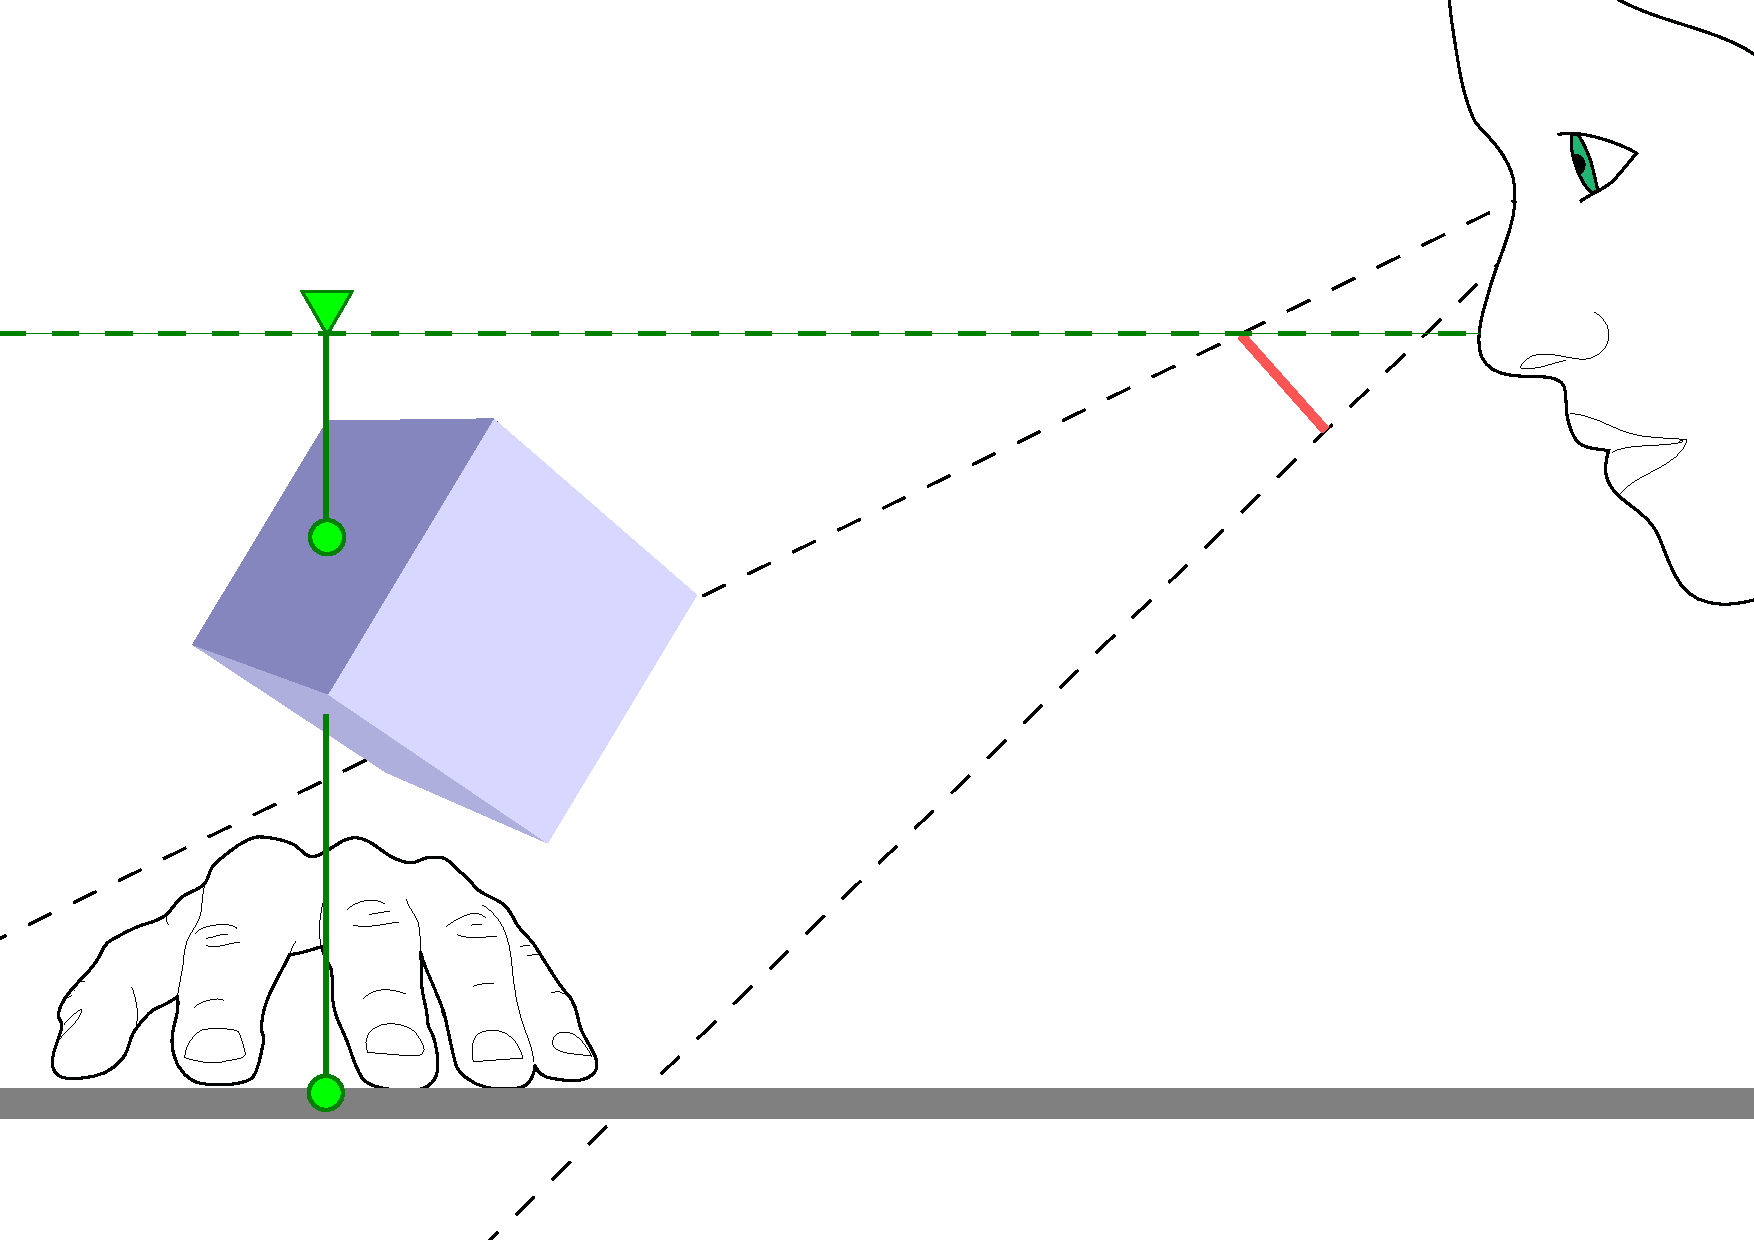
\includegraphics[width=12cm]{img/intersection_lift.pdf}
	\end{center}
	\caption{Anhebung des Startpunkts (grünes Dreieck) auf Höhe der \emph{Near Clipping Plane} (rot) für den Schnitttest (grün) bei der \emph{Levelling} Interaktion.} 
	\label{fig:intersection_lift}
\end{figure}

Die Punkte auf der Geometrie werden durch einen Schnitttest ausgehend vom jeweiligen Eingabepunkt auf dem Tisch und entlang der Bildschirmnormalen ermittelt. Bei der Schnittberechnung ist wichtig, dass negativ parallaxe Modellbereiche nicht übersehen werden. Folglich muss die z-Koordinate des Startpunkts für den Schnittstrahl\footnote{im Screenspace} auf die Höhe der \emph{Near-Clipping-Plane} angehoben werden. Abbildung \ref{fig:intersection_lift} veranschaulicht diesen Zusammenhang.
\\\\
Wir definieren \emph{Touch-Kontakte} als Strukturen, welche sowohl den Eingabepunkt auf dem Bildschirm, als auch den zugehörigen Geometrieschnittpunkt beinhaltet. Die Orthogonalität der Verbindungsgeraden von Bildschirm- und Geometriepunkt eines \emph{Touch-Kontakts} soll während der Interaktion mit dem Tisch erhalten bleiben. Um dies zu erreichen, muss \emph{Levelling} der Anwendung von RTS im Bildraum (siehe \ref{sec:rst_im_bildraum}) beigefügt werden. Wir nennen diesen Modus Rotation, Translation und Skalierung im Bildraum, erweitert durch \emph{Levelling} (RTS+L).


\section{Depth-Levelling}
\label{sec:depth_levelling}

\emph{Depth-Levelling} wird durch das Eingeben zweier \emph{Touch-Kontakte} initiiert. Nach der Schnittberechnung erfolgt die Einordnung dieser in \emph{Primär-} und \emph{Sekundärkontakt}. Der Geometrieschnittpunkt des \emph{Primärkontakts} liegt näher an der Tischebene oder ist weiter über der dieser als der des \emph{Sekundärkontakts}. Ziel des \emph{Depth-Levellings} ist es, den Geometriereferenzpunkt des \emph{Primärkontakts} durch Translation auf die Projektionsebene zu bringen. Um dies zu erreichen wird das Viewing Setup schrittweise entlang der Bildschirmnormalen verschoben. 
\\\\
Die Schrittweite der Translation wird bei RTS+L durch einen Faktor festgelegt welcher aus der Relation zwischen den \emph{Touch-Kontakten} abgeleitet ist. Ist die Geometrie bereits in relativer Bildschirmnähe, bietet sich die Differenz der Distanz zwischen den Eingabepunkten  seit der letzten Interaktion an. Demnach ist die Levelling-Distanz ($t_L$) gegeben durch:
\\\\
$t_L = | (|V_{S_1S_2}|) - (|V_{S_1S_2}‘|) |$ 
\\\\
,wobei $V_{S_1S_2}$ der Vektor zwischen den Bildschirmpunkten der Touch-Kontakte vor der Eingabe ist und $V_{S_1S_2}‘$ danach. 
\\\\
Für eine größere Translationsdistanz bei weit von der Bildfläche entfernten Objekten, kann stattdessen das Verhältnis der Länge zwischen $V_{S_1S_2}$ und $V_{S_1S_2}‘$ zur Berechnung von $t_L$ genutzt werden.
\\\\
$t_L = \left||G| - |G| * \frac{|V_{S_1S_2}|}{|V_{S_1S_2}‘|}\right|$
\\\\
,wobei $G$ der Richtungsvektor zwischen dem Geometrieschnittpunkt des Primärkontakts und dessen Punkt auf dem Bildschirm ist.
\\\\
Sollte die nach einem der genannten Ansätze ermittelte \emph{Levelling}-Distanz größer oder gleich der Länge des Richtungsvektors zwischen dem Geometrie- und dem Bildschirmpunkt des \emph{Primärkontakts} sein, so wird stattdessen eine Translation um diesen Vektor angewandt. Nach dieser Bewegung befindet sich der Geometriereferenzpunkt des \emph{Primärkontakts} auf Tischebene und das \emph{Depth-Levelling} ist beendet.

\section{Rotation-Levelling}
\label{sec:rotation_levelling}

Das \emph{Rotation-Levelling} schließt sich an die Durchführung des \emph{Depth-Levellings} an. Dieser Vorgang dient der Heranführung des Geometrieschnittpunkts des Sekundärkontakts an die Projektionsebene. Der Modellschnittpunkt des \emph{Primärkontakts} würde durch Translation von der Bildschirmebene entfernt werden. Dies führt zur Aufhebung des durch \emph{Depth-Levelling} erreichten Interaktionsziels. Stattdessen wird eine Rotation um den Bildschirmpunkt des \emph{Primärkontakts} vorgenommen. Des Weiteren muss eine Skalierung in Richtung des selbigen Referenzpunkt erfolgen. Mit diesem Schritt soll gewährleistet werden, dass der Richtungsvektor zwischen Geometrie- und Bildschirmpunkt des \emph{Sekundärkontakts} weiterhin senkrecht auf der Bildebene steht.
\\\\
Die Parametrisierung der Rotation bestimmt sich wie folgt.  Sei $G_2$ der Geometrieschnittpunkt des \emph{Sekundärkontakts} und $S_2$ der zugehörige Punkt der Eingabe auf dem Bildschirm, so bestimmt sich $V_{G_2S_2}$ als Richtungsvektor zwischen $G_2$ und $S_2$. Wie beim \emph{Depth-Levelling} (siehe Abschnitt \ref{sec:depth_levelling}) wird im ersten Schritt der Distanzfaktor ($t_L$) für Annäherung an die Bildebene ermittelt. Danach wird ein Punkt $G_2‘$ berechnet, der die Position von $G_2$ nach Verschiebung um $t_L$ entlang $V_{G_2S_2}$ beschreibt. Als nächstes werden zwei Vektoren $V_{S_1G_2}$ und $V_{S_1G_2‘}$ bestimmt. $V_{S_1G_2}$ ist hierbei der Richtungsvektor zwischen dem zugehörigen Bildschirmpunkt des \emph{Primärkontakts} $S_1$ und $G_2$. $V_{S_1G_2‘}$ ist der Richtungsvektor zwischen $S_1$ und $G_2‘$. Der Rotationswinkel ($\alpha_L$) und die Rotationsachse ($R_L = (x, y, z)$) ergeben sich aus:
\\\\
$\alpha_L = arccos(||V_{S_1G_2}|| * || V_{S_1G_2‘}||)$
\\
$R_L = ||V_{S_1G_2}|| \times ||V_{S_1G_2‘}||$ 
\\\\
Wie bereits erwähnt dient eine Skalierung in Richtung des Geometriepunkts des \emph{Primärkontakts} zum Erhalt der Orthogonalität zwischen Geometrie- und Bildschirmpunkt des \emph{Sekundärkontakts}. Der Skalierungsfaktor ($S_L$) ist gegeben durch:
\\\\
$S_L = \frac{|V_{S_1G_2}|}{|V_{S_1G_2‘}|}$
\\\\
Befindet sich der Geometrieschnittpunkt des \emph{Sekundärkontaks} nach Anwendung aller Transformationen auf der Bildebene, so ist das Interaktionsziel erreicht und das \emph{Rotation-Levelling} beendet.


\section{Vorteile und Limitierungen}
\label{sec:vorteile_und_limitierungen_implizit}

\begin{figure}
	\begin{center}
		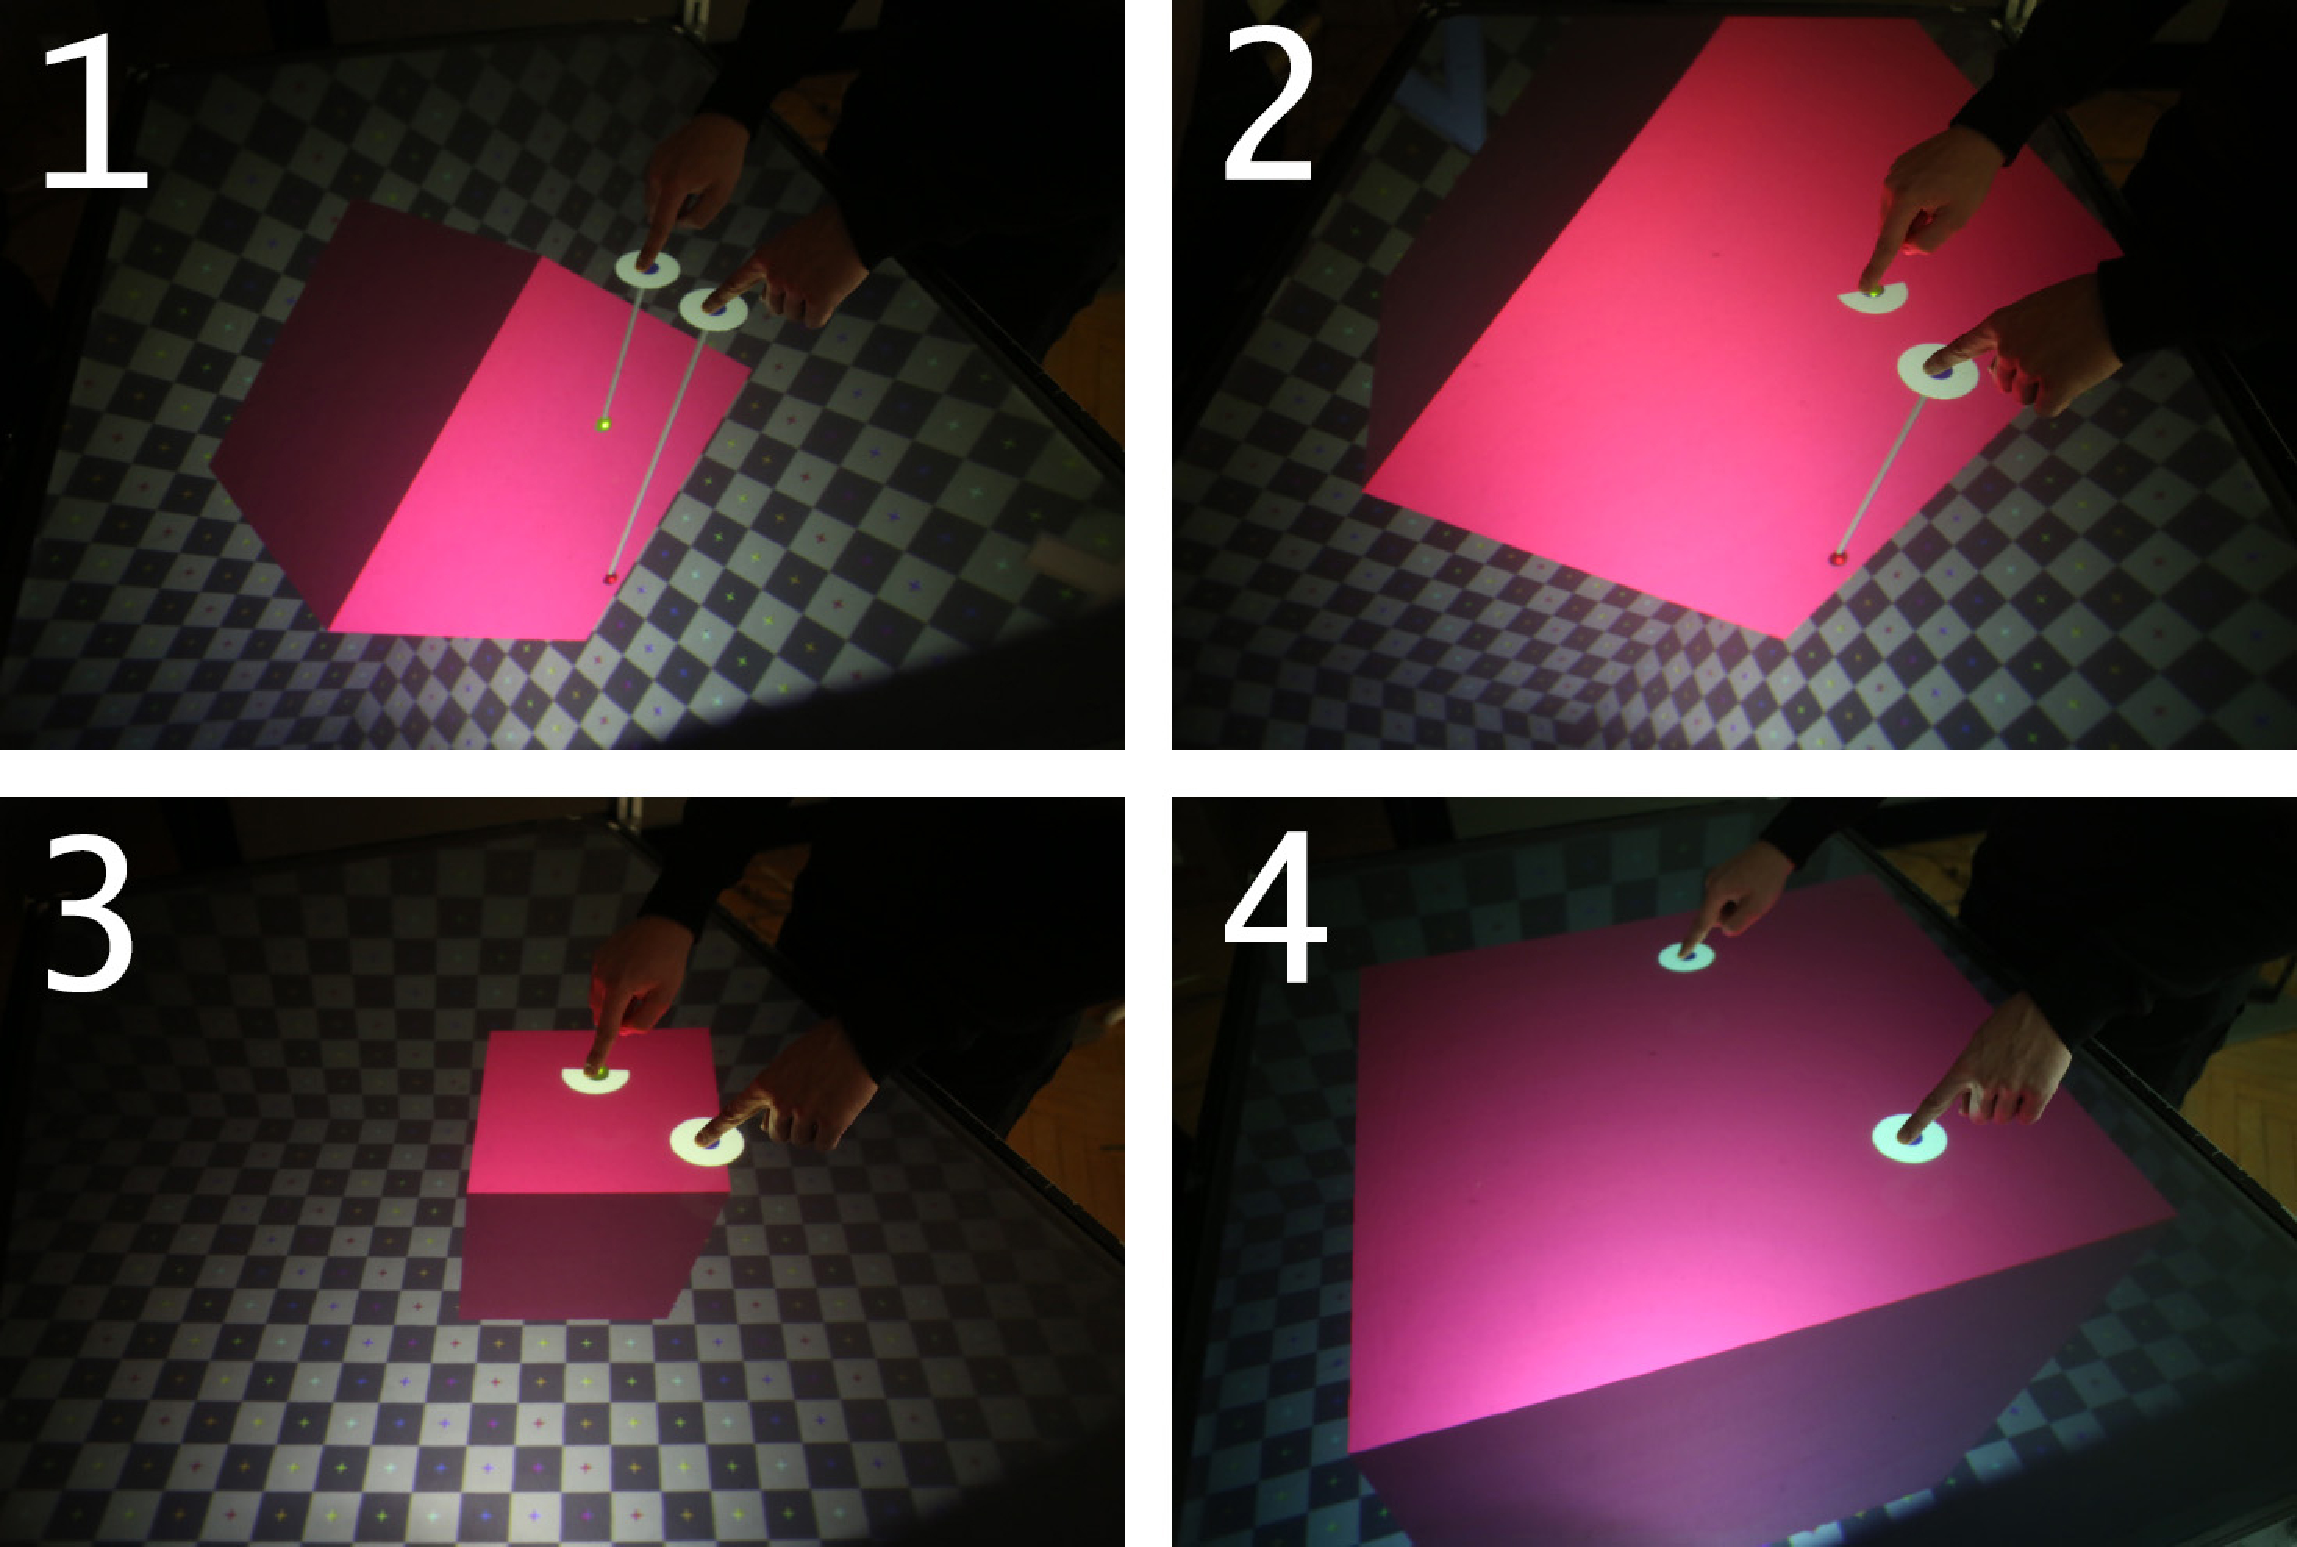
\includegraphics[width=10cm]{img/levelling_lock.pdf}
	\end{center}
	\caption{Ablauf einer \emph{Levelling} Interaktion. Bild 1 zeigt die ermittelten Orthogonalschnittpunkte mit der Szenengeometrie. In Bild 2 hat der Geometrieschnittpunkt des \emph{Primärkontakts} durch \emph{Depth-Levelling} die Bildebene erreicht. Bild 3 zeigt die Ebnung des Sekundärschnittpunkts durch \emph{Rotation-Levelling}. Danach sind lediglich RST Manipulationen möglich, wie Bild 4 verdeutlicht.}
	\label{fig:levelling_lock}
\end{figure}

Das am Lehrstuhl entwickelte Point Based Rendering  System ermöglicht die Analyse von komplexen 3D Oberflächen-Scans in einem großen Umfang verschiedener Auflösungsstufen. Nach den in Abschnitt \ref{sec:multi_touch_interaktion_mit_3d_szenen} beschriebenen Konzepten, ist die Betrachtung und Interaktion mit dreidimensionalen Modellen vor allem in Bereichen nahe der Projektionseben effektiv möglich. Aus diesem Zusammenhang leitet sich das Interaktionsziel, nutzerdefinierte Inhalte in Bildschirmnähe zu bringen, ab. Durch Anwendung von RTS+L wird der Nutzer ohne Einführung neuer Gesten bei der Erreichung dieses Ziels unterstützt. Hierbei wird die Komplexität der zur Manipulation erforderlichen Transformation vor dem Anwender verborgen.
\\\\
\emph{Levelling} ist als implizite Navigationstechnik nach RTS+L nicht ohne den Einfluss von RTS bedienbar. Umgekehrt betrachtet können Rotation, Translation und Skalierung bei RTS+L nur getrennt von \emph{Levelling} bedient werden, wenn sich die Geometrieschnittpunkte beider \emph{Touch-Kontakte} auf der Bildebene befinden. 
\\\\
Die am schwersten wiegende Limitierung ist, dass die durch \emph{Levelling} hervorgerufene Manipulation bei RTS+L nicht umkehrbar ist. Demnach schließt RTS+L zwar die z-Translation, sowie 3D Rotation ein, jedoch nur in Richtung der durch die \emph{Touch-Kontakte} definierten Vektoren. Abbildung \ref{fig:levelling_lock} zeigt ein einfaches Beispiel der Folge dieses Problems. Hier wird ein Würfel unter der Tischebene positioniert. Nach mehrmaligem Anwenden liegt eine der Flächen der Geometrie in der Bildebene. Eine weitere Manipulation durch \emph{Levelling} ist nicht möglich, da sich die Seitenflächen der Würfel orthogonal zur Bildebene befinden. Die gegenüberliegende Fläche ist durch die in der Projektionsebene liegende verdeckt und wird daher vom Geometrieschnitttest bei der Initiierung der Geste nicht getroffen.